\documentclass[16pt]{report}
\usepackage[utf8]{inputenc}
\usepackage[russian]{babel}

\usepackage{indentfirst}
\usepackage{amsmath}
\usepackage{graphicx}
\usepackage{listings}
\usepackage{biblatex}
\usepackage{float}
\usepackage{floatrow}
\usepackage{caption}
\usepackage{mathtools}
\usepackage{setspace}

\addbibresource{report.bib}

\usepackage{etoolbox}
\makeatletter
\patchcmd{\chapter}{\if@openright\cleardoublepage\else\clearpage\fi}{}{}{}
\makeatother

\lstset{extendedchars=\true, frame=single, numbers=left,captionpos=t}

\usepackage[left=2cm,right=2cm, top=2cm,bottom=2cm,bindingoffset=0cm]{geometry}
\usepackage{titlesec, blindtext, color}
\newcommand{\hsp}{\hspace{20pt}}
\titleformat{\chapter}[hang]{\Huge\bfseries}{\thechapter\hsp{|}\hsp}{0pt}{\Huge\bfseries}

\begin{document}
\def\chaptername{}
\thispagestyle{empty}
\begin{titlepage}
	\noindent \begin{minipage}{0.15\textwidth}
	
\includegraphics[width=\linewidth]{img/bmstu.jpg}
	\end{minipage}
	\noindent\begin{minipage}{0.9\textwidth}\centering
		\textbf{Министерство науки и высшего образования Российской Федерации}\\
		\textbf{Федеральное государственное бюджетное образовательное учреждение высшего образования}\\
		\textbf{~~~«Московский государственный технический университет имени Н.Э.~Баумана}\\
		\textbf{(национальный исследовательский университет)»}\\
		\textbf{(МГТУ им. Н.Э.~Баумана)}
	\end{minipage}
	
	\noindent\rule{18cm}{3pt}
	\newline\newline
	\noindent ФАКУЛЬТЕТ $\underline{\text{«Информатика и системы управления»}}$ \newline\newline
	\noindent КАФЕДРА $\underline{\text{«Программное обеспечение ЭВМ и информационные технологии»}}$\newline\newline\newline\newline\newline
	
	
	\begin{center}
		\noindent\begin{minipage}{1.3\textwidth}\centering
			\Large\textbf{  Отчет по лабораторной работе №6}\newline
			\textbf{по дисциплине "Моделирование"}\newline
			\newline\newline\newline
		\end{minipage}
	\end{center}
	
	\noindent\textbf{Тема} $\underline{\text{~~~~~~~~~Моделирование склада~~~~~~~~~~}}$\newline\newline
	\noindent\textbf{Студент} $\underline{\text{~~~~~Костев Д. И.~~~~~~}}$\newline\newline
	\noindent\textbf{Группа} $\underline{\text{~~~~~~~~~~ИУ7-71Б~~~~~~~~~~}}$\newline\newline
	\noindent\textbf{Оценка (баллы)} $\underline{\text{~~~~~~~~~~~~~~~~~~~~~~~~~~~~~}}$\newline\newline
	\noindent\textbf{Преподаватель} $\underline{\text{~~~Рудаков И. В.~~~~~~~~}}$\newline\newline\newline
	
	\begin{center}
		\vfill
		Москва~---~\the\year
		~г.
	\end{center}
\end{titlepage}

\newpage

\chapter*{Задача}
{\LargeРеализовать программу для моделирования следующей системы: товар поступает на обработку с интервалами $\SI{4}{} \pm \SI{2}{}$ минуты. Оператор направляет товар в очередь к наименее нагруженному упаковщику. Каждый упаковщик работает $\SI{10}{} \pm \SI{5}{}$ минут. Далее упакованный товар распределяется к наименее нагруженному фасовщику. Фасовщики относят товар на необходимые полки в течение  $\SI{6}{} \pm \SI{3}{}$ минут.\\ 


Возьмем следующее количество работников:

\begin{itemize}
  \item 4 упаковщика
  \item 3 фасовщика 
\end{itemize}

\section*{}
\begin{figure}[h]
	\centering
	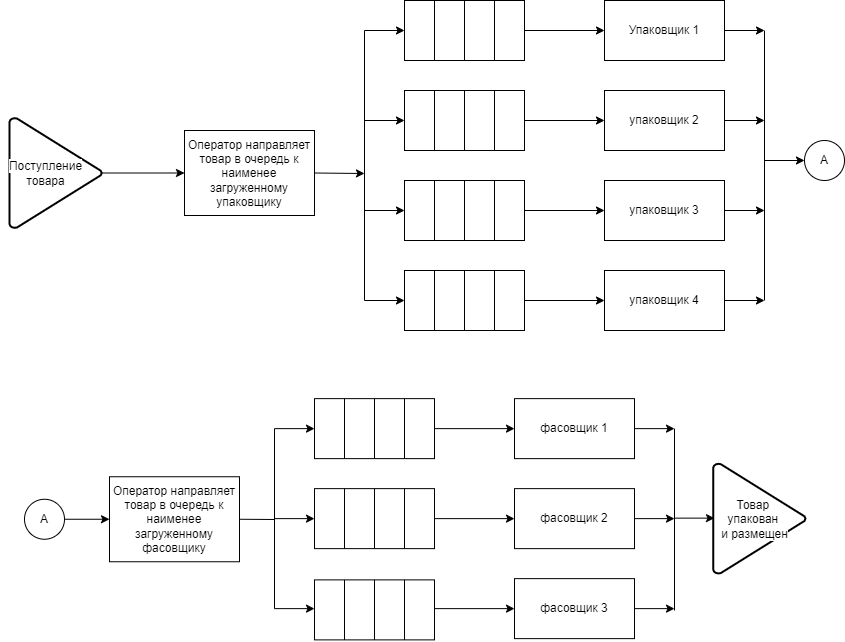
\includegraphics[scale=0.4]{diag-Page-1.drawio.png}
	\label{fig:screenshot001}
\end{figure}
} 



\newpage
\chapter{Результаты работы}
{\Large100 заявок:}
\begin{figure}[h]
	\centering
	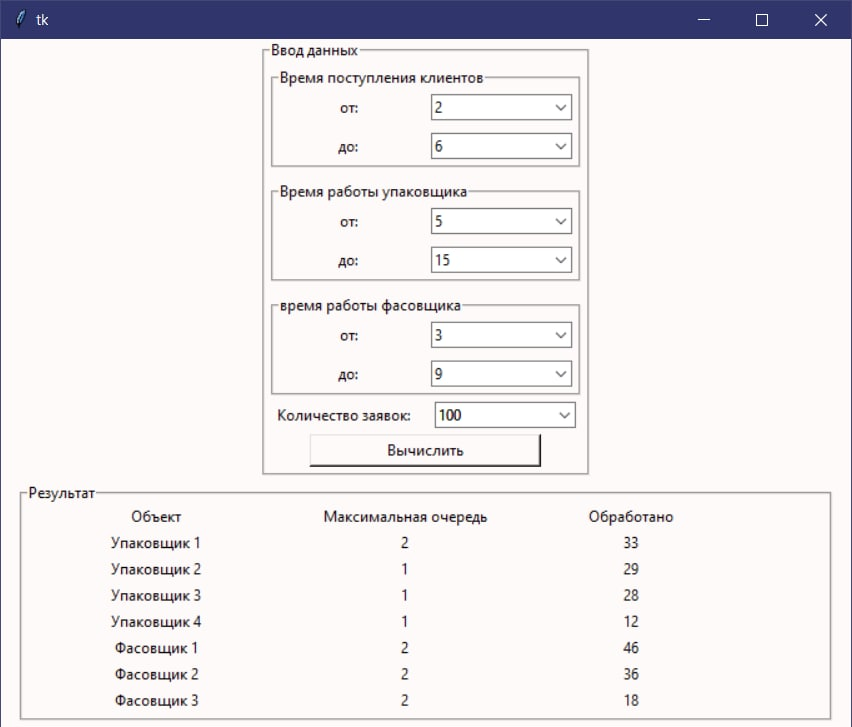
\includegraphics[scale=0.8]{1.jpg}
	\label{fig:screenshot001}
\end{figure}
\newpage
{\Large300 заявок:}
\begin{figure}[h]
	\centering
	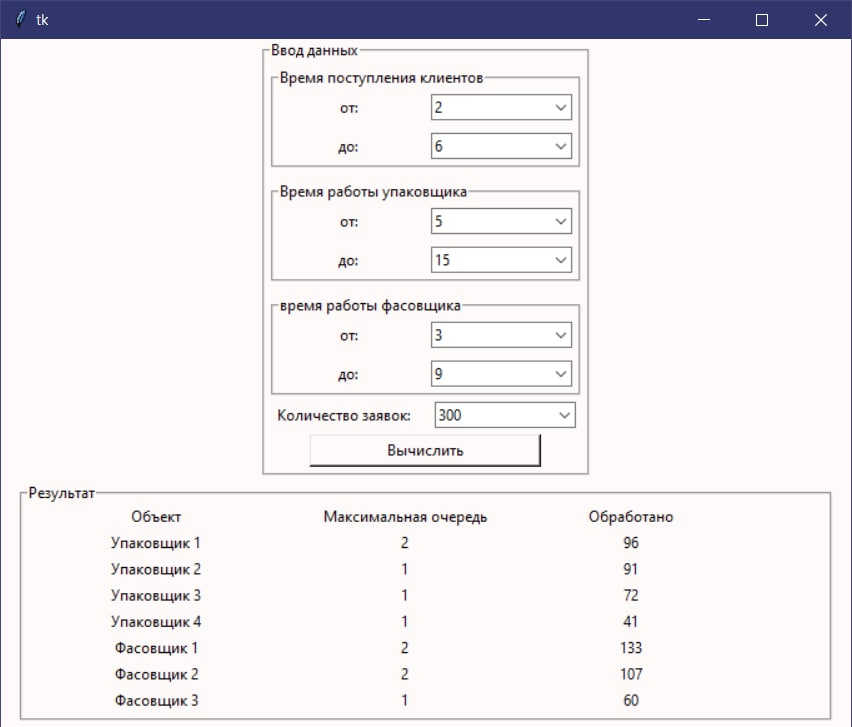
\includegraphics[scale=0.8]{2.jpg}
	\label{fig:screenshot001}
\end{figure}
\newpage
{\Large1000 заявок:}
\begin{figure}[h]
	\centering
	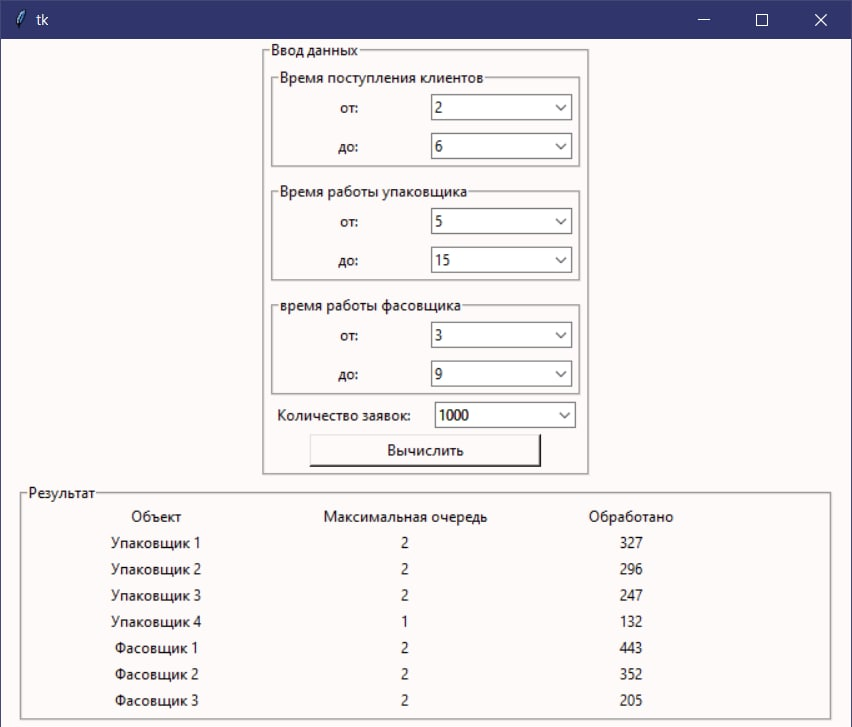
\includegraphics[scale=0.8]{3.jpg}
	\label{fig:screenshot001}
\end{figure}
\newpage
{\Large3000 заявок:}
\begin{figure}[h]
	\centering
	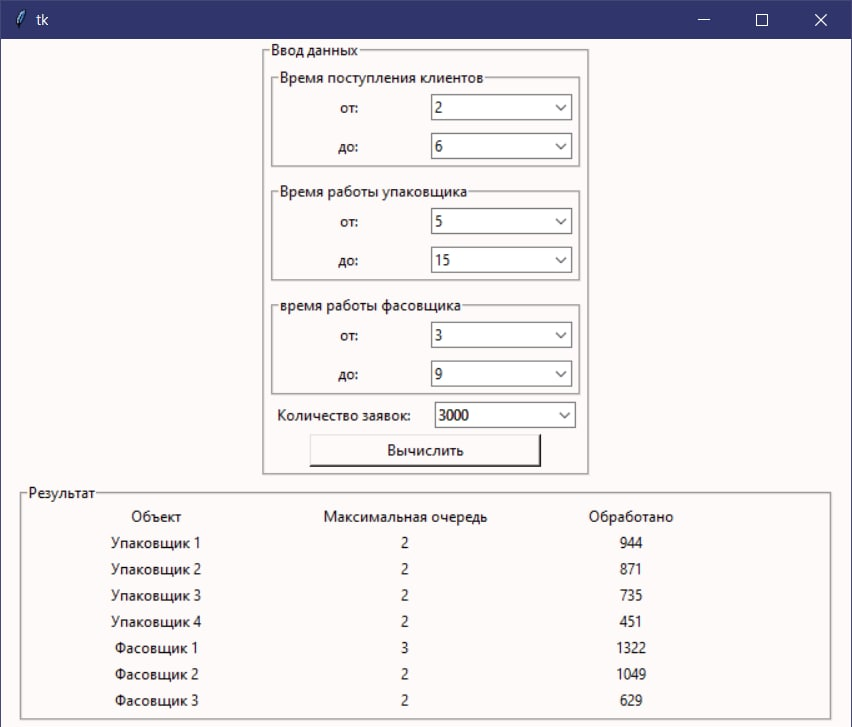
\includegraphics[scale=0.8]{4.jpg}
	\label{fig:screenshot001}
\end{figure}
\newpage
{\Large10000 заявок:}
\begin{figure}[h]
	\centering
	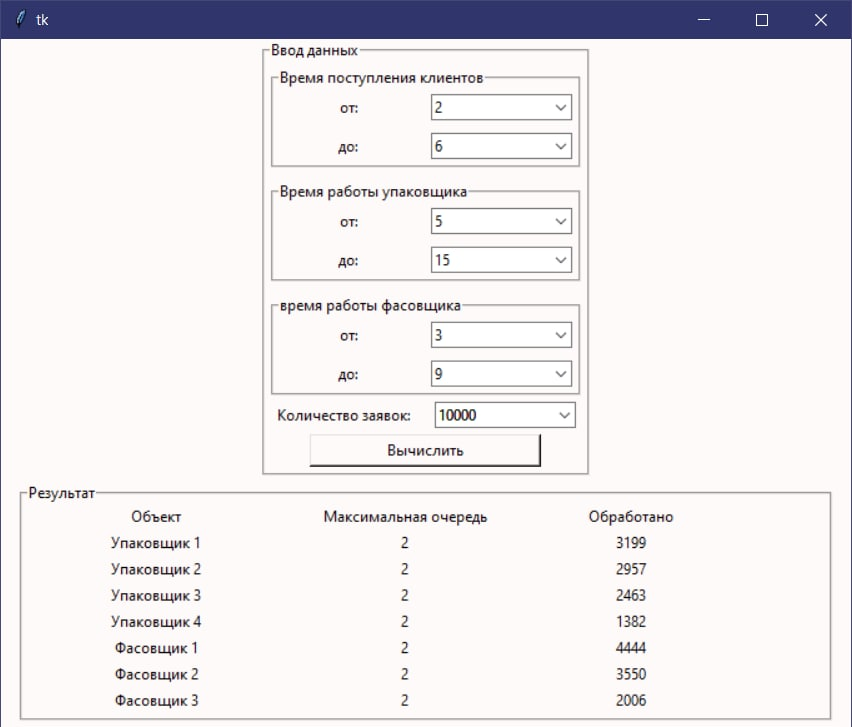
\includegraphics[scale=0.8]{5.jpg}
	\label{fig:screenshot001}
\end{figure}

\chapter*{Вывод}
\begin{doublespace}
{\Large Таким образом, видно, что количество работников отпимально для продуктивного выполнения работы так, чтобы товары не накапливались в очередях и быстро оказывались на полках.}
\end{doublespace}

\end{document} 